\documentclass[11pt,a4paper]{article}
 
% -----------------------------------------------------------------------
% Packages
% -----------------------------------------------------------------------
\usepackage[margin=1.25in]{geometry}
\usepackage{amsmath,amssymb,amsthm}
\usepackage{mathtools}
\usepackage{algorithm}
\usepackage{algpseudocode}
\usepackage{booktabs}
\usepackage{graphicx}
\usepackage{hyperref}
\usepackage{xcolor}
\usepackage{microtype}
\usepackage{natbib}
\usepackage{setspace}
\usepackage{parskip}
 
% arXiv-style header tweaks
\hypersetup{
  colorlinks = true,
  linkcolor  = {blue!60!black},
  citecolor  = {blue!60!black},
  urlcolor   = {blue!60!black},
}
 
% -----------------------------------------------------------------------
% Theorem environments
% -----------------------------------------------------------------------
\newtheorem{remark}{Remark}
\newtheorem{proposition}{Proposition}
 
% -----------------------------------------------------------------------
% Notation shorthands
% -----------------------------------------------------------------------
\newcommand{\R}{\mathbb{R}}
\newcommand{\E}{\mathbb{E}}
\newcommand{\Prob}{\mathbb{P}}
\newcommand{\N}{\mathcal{N}}
\newcommand{\D}{\mathcal{D}}
\newcommand{\dt}{\,\mathrm{d}t}
\newcommand{\dW}{\,\mathrm{d}W}
\newcommand{\given}{\,|\,}
\newcommand{\iid}{\overset{\text{iid}}{\sim}}
\newcommand{\psup}{p_{\text{sup}}}
\newcommand{\thetaT}{\theta_T}
\newcommand{\thetaC}{\theta_C}
\newcommand{\etaE}{\eta_E}
\newcommand{\etaF}{\eta_F}
 
% -----------------------------------------------------------------------
\begin{document}
% -----------------------------------------------------------------------
 
% ---- Title block -------------------------------------------------------
\begin{center}
  {\LARGE \textbf{Bayesian Adaptive Clinical Trial Simulation}}\\[0.6em]
  {\large Stochastic Disease Progression, Sequential Bayesian Inference,}\\
  {\large and Response-Adaptive Randomisation}\\[1.2em]
  {\normalsize Jesse Koivu, PhD Mathematics}\\[0.4em]
  {\small \today}
\end{center}
 
\vspace{0.5em}
\hrule
\vspace{1em}
 
% ---- Abstract ----------------------------------------------------------
\begin{abstract}
We present a three-layer simulation framework for a Phase~II oncology
adaptive clinical trial.
Layer~1 models tumour burden as a Gompertz stochastic differential equation
(SDE) with multiplicative noise, calibrated to published tumour-growth-inhibition
(TGI) parameters and discretised via the Milstein scheme.
Layer~2 performs sequential Bayesian inference on objective response rates
using a Beta-Binomial model with conjugate posteriors; a full MCMC
implementation via PyMC with the No-U-Turn Sampler (NUTS) is provided for
final-analysis diagnostics.
Layer~3 wraps Layers~1--2 into an adaptive trial engine: response-adaptive
randomisation (RAR) via Thompson sampling updates the patient allocation ratio
at each interim look, and Bayesian stopping rules terminate the trial early for
efficacy or futility.
Operating characteristics---power, Type~I error, expected sample size, and
early-stop rate---are estimated by Monte Carlo simulation over a grid of true
treatment effects.
The adaptive design assigns approximately 60--67\% of enrolled patients to the
superior treatment arm at moderate effect sizes, compared to 50\% under fixed
1:1 randomisation, at comparable statistical power.
\end{abstract}
 
\vspace{1em}
\hrule
\vspace{1em}
 
\tableofcontents
 
\newpage
 
% ========================================================================
\section{Introduction}
% ========================================================================
 
Standard randomised controlled trials fix the allocation ratio and sample size
at design time. This is statistically clean but ethically inefficient: if
interim data strongly suggest one arm is superior, a fixed design continues
enrolling patients onto the inferior arm regardless. Adaptive designs address
this by allowing the trial to respond to accumulating evidence---stopping early
when the posterior probability of superiority crosses a pre-specified threshold,
and redistributing allocation toward the better-performing arm in real time.
 
Bayesian adaptive designs are increasingly prominent in oncology and rare-disease
trials. High-profile examples include I-SPY2 (breast cancer, multi-arm),
BATTLE (lung cancer, biomarker-adaptive), and GBM AGILE (glioblastoma). The
US Food and Drug Administration issued dedicated guidance in 2019~\cite{FDA2019}.
Despite this, their operating characteristics (OC) remain poorly understood by
practitioners without a simulation-based grounding: unlike frequentist designs
where sample size and power are analytically tractable, adaptive designs require
Monte Carlo estimation.
 
This project builds that grounding from first principles. The three-layer
architecture separates biological simulation, statistical inference, and
sequential decision-making into independent, testable modules, connected by a
clean data interface. The goal is both methodological---demonstrating that the
SDE and Bayesian inference layers are correctly specified---and practical,
producing an OC surface that a trial statistician could use to argue for or
against a specific adaptive design.
 
\paragraph{Contributions.}
\begin{itemize}
  \item A biologically motivated Gompertz SDE simulator calibrated to published
        TGI parameters, with Milstein discretisation and RECIST~1.1 response
        classification.
  \item A two-path Bayesian inference engine: a conjugate closed-form path for
        real-time interim updates, and a PyMC NUTS path for final-analysis
        diagnostics with R-hat and ESS validation.
  \item A Thompson sampling RAR engine with clipped allocation, Bayesian
        stopping rules, and a Monte Carlo OC surface across a treatment-effect
        grid.
  \item A prior sensitivity analysis quantifying the impact of sceptical,
        neutral, and optimistic priors on stopping decisions at each interim look.
\end{itemize}
 
% ========================================================================
\section{Statistical Model}
% ========================================================================
 
\subsection{Layer~1: Tumour Dynamics (Gompertz SDE)}
\label{sec:layer1}
 
\subsubsection{Model specification}
 
Tumour volume $V(t) \in \R_{>0}$ at time $t \geq 0$ is modelled by the
Gompertz SDE:
\begin{equation}
  \label{eq:gompertz-sde}
  \mathrm{d}V(t)
  = \bigl[\alpha - \beta \ln V(t) - \delta\bigr]\,V(t)\dt
  + \sigma\,V(t)\dW(t),
\end{equation}
where $W(t)$ is a standard Brownian motion on a filtered probability space
$(\Omega, \mathcal{F}, (\mathcal{F}_t)_{t\geq 0}, \Prob)$, and the
parameters are:
\begin{itemize}
  \item $\alpha > 0$: intrinsic proliferation rate (day$^{-1}$),
  \item $\beta > 0$: Gompertz deceleration coefficient (day$^{-1}$), encoding
        vascular and nutrient limitation,
  \item $\delta \geq 0$: drug-induced elimination rate (day$^{-1}$); $\delta = 0$
        in the control arm,
  \item $\sigma > 0$: diffusion coefficient (day$^{-1/2}$), encoding biological
        noise.
\end{itemize}
 
The drift $\mu(V) = [\alpha - \beta \ln V - \delta]\,V$ encodes three competing
forces: exponential proliferation ($\alpha V$), Gompertz braking ($-\beta V \ln V$),
and cytotoxic kill ($-\delta V$). The noise term $\sigma V\,\mathrm{d}W$ is
\emph{multiplicative}: noise scales proportionally with tumour volume, which
preserves $V(t) > 0$ almost surely and implies a constant coefficient of
variation across all tumour sizes. This is consistent with the TGI model class
validated against clinical RECIST data by Stein et al.~\cite{Stein2011} and
Claret et al.~\cite{Claret2013}.
 
\begin{remark}[Gompertz vs.\ logistic growth]
Both Gompertz and logistic models include a carrying capacity, but they differ
in the trajectory of deceleration. The logistic model decelerates symmetrically
around half the carrying capacity; the Gompertz model decelerates earlier and
more steeply. Empirically, solid tumour data exhibit early deceleration more
consistent with Gompertz kinetics~\cite{Stein2011}. Under the calibrated
parameters the carrying capacity is $\exp(\alpha/\beta) \approx 790\;\text{cm}^3$,
representing a tumour that would be fatal untreated.
\end{remark}
 
\subsubsection{Milstein discretisation}
 
Let $\Delta t$ denote the time step and $\Delta W_k \sim \N(0, \Delta t)$
independently for each step $k$. The plain Euler--Maruyama scheme gives
strong convergence of order $\tfrac{1}{2}$. For the multiplicative diffusion
$g(V) = \sigma V$ the Milstein correction~\cite{Kloeden1992} adds a term
involving $g \cdot g' = \sigma^2 V$, raising the strong order to~1:
 
\begin{equation}
  \label{eq:milstein}
  V_{k+1} = V_k
  + \bigl[\alpha - \beta \ln V_k - \delta\bigr] V_k \,\Delta t
  + \sigma V_k \,\Delta W_k
  + \tfrac{1}{2}\,\sigma^2 V_k \bigl(\Delta W_k^2 - \Delta t\bigr).
\end{equation}
 
A reflecting lower boundary at $V_{\min} = 10^{-4}\;\text{cm}^3$ prevents
numerical underflow. The step size $\Delta t = 0.5$ days satisfies
$\sigma\sqrt{\Delta t} \approx 0.042 \ll 1$, ensuring the Milstein scheme
operates in its convergence regime.
 
\subsubsection{Baseline heterogeneity}
 
Patient baseline volumes $V_0$ are drawn independently from a log-normal
distribution:
\begin{equation}
  \ln V_0 \sim \N\!\left(\mu_\ell,\, \sigma_\ell^2\right),
  \quad
  \mu_\ell = \ln \bar{V}_0 - \tfrac{1}{2}\ln(1 + c^2),
  \quad
  \sigma_\ell = \sqrt{\ln(1+c^2)},
\end{equation}
with mean $\bar{V}_0 = 25\;\text{cm}^3$ and coefficient of variation $c = 0.50$,
reflecting the wide variation in tumour burden at trial entry in an unselected
Phase~II population.
 
\subsubsection{RECIST~1.1 response classification}
 
At the primary assessment time $T_{\text{assess}} = 84$ days (12~weeks), each
patient $i$ is classified by their percentage change from baseline
$\Delta_i = (V_i(T_{\text{assess}}) - V_{0,i})\,/\,V_{0,i}$:
 
\begin{equation}
  R_i =
  \begin{cases}
    \text{CR} & \text{if } \Delta_i \leq -1.00 \\
    \text{PR} & \text{if } -1.00 < \Delta_i \leq -0.30 \\
    \text{SD} & \text{if } -0.30 < \Delta_i < +0.20 \\
    \text{PD} & \text{if } \Delta_i \geq +0.20.
  \end{cases}
\end{equation}
 
The binary endpoint for Layer~2 is objective response (OR $= \mathbf{1}[R_i \in
\{\text{CR, PR}\}]$), giving the objective response rate
$\text{ORR} = n^{-1}\sum_i \mathbf{1}[R_i \in \{\text{CR, PR}\}]$.
 
\subsubsection{Calibrated parameters}
 
Default parameters are anchored to Stein et al.~\cite{Stein2011}:
 
\begin{table}[h]
\centering
\begin{tabular}{@{}llll@{}}
\toprule
Parameter & Symbol & Value & Interpretation \\
\midrule
Proliferation rate    & $\alpha$             & $0.012\;\text{day}^{-1}$  & Intrinsic growth \\
Gompertz coeff.       & $\beta$              & $0.0018\;\text{day}^{-1}$ & Vascular limitation \\
Noise coefficient     & $\sigma$             & $0.06\;\text{day}^{-1/2}$ & Biological variability \\
Drug effect (treat.)  & $\delta_T$           & $0.005$--$0.011\;\text{day}^{-1}$ & OC grid \\
Drug effect (ctrl.)   & $\delta_C$           & $0.001\;\text{day}^{-1}$  & Residual decay (BSC) \\
Baseline volume       & $\bar{V}_0$          & $25\;\text{cm}^3$         & Log-normal mean \\
Baseline CV           & $c$                  & $0.50$                    & Patient heterogeneity \\
SDE step              & $\Delta t$           & $0.5\;\text{days}$        & Milstein step \\
Assessment time       & $T_{\text{assess}}$  & $84\;\text{days}$         & RECIST 12-week read \\
\bottomrule
\end{tabular}
\caption{Default SDE parameters calibrated to Stein et al.~\cite{Stein2011}.
At $\delta_T = 0.009$ the model produces treatment ORR $\approx 44\%$ vs.\
control ORR $\approx 14\%$, consistent with a positive Phase~II result in a
solid tumour setting.}
\label{tab:params}
\end{table}
 
% -----------------------------------------------------------------------
\subsection{Layer~2: Bayesian Response Model}
\label{sec:layer2}
 
\subsubsection{Likelihood and conjugate posterior}
 
Let $y_a$ denote the number of responders among $n_a$ patients in arm
$a \in \{T, C\}$. We model response rates $\theta_a \in (0,1)$ via the
Beta-Binomial model:
\begin{align}
  y_a \given \theta_a &\sim \text{Binomial}(n_a,\, \theta_a), \label{eq:likelihood} \\
  \theta_a             &\sim \text{Beta}(\alpha_a,\, \beta_a). \label{eq:prior}
\end{align}
 
By conjugacy the posterior is available in closed form:
\begin{equation}
  \label{eq:posterior}
  \theta_a \given y_a \;\sim\; \text{Beta}(\alpha_a + y_a,\;\; \beta_a + n_a - y_a).
\end{equation}
 
The posterior mean is $\hat{\theta}_a = (\alpha_a + y_a)/(\alpha_a + \beta_a + n_a)$,
which shrinks the MLE $y_a/n_a$ toward the prior mean $\alpha_a/(\alpha_a+\beta_a)$
with strength proportional to the prior effective sample size
$\text{ESS} = \alpha_a + \beta_a$.
 
\subsubsection{Decision quantity}
 
The primary decision quantity at each interim look is the posterior probability
of treatment superiority:
\begin{equation}
  \label{eq:psup}
  \psup
  = \Prob(\thetaT > \thetaC \given \mathcal{D})
  = \int_0^1 F_C(\theta)\,p_T(\theta)\,\mathrm{d}\theta,
\end{equation}
where $F_C$ is the posterior CDF of $\thetaC$ and $p_T$ is the posterior
density of $\thetaT$. This integral has no simple closed form, so $\psup$
is estimated by Monte Carlo:
\begin{equation}
  \hat{p}_{\text{sup}}
  = \frac{1}{S}\sum_{s=1}^{S}
    \mathbf{1}\!\left[\thetaT^{(s)} > \thetaC^{(s)}\right],
  \quad
  \thetaT^{(s)} \iid p_T,\;
  \thetaC^{(s)} \iid p_C,
\end{equation}
with $S = 50{,}000$ draws. A secondary quantity is the probability of a
clinically meaningful difference:
\begin{equation}
  \label{eq:pmid}
  p_{\text{MID}} = \Prob(\thetaT - \thetaC > \Delta_{\min} \given \mathcal{D}),
\end{equation}
with minimum important difference $\Delta_{\min} = 0.10$.
 
\subsubsection{Prior specification and sensitivity}
 
The control prior is fixed across all analyses, anchored to a historical
control ORR of 15\%: $\thetaC \sim \text{Beta}(3, 17)$, giving
$\E[\thetaC] = 0.15$ and $\text{ESS} = 20$. Three treatment prior regimes
encode different states of knowledge:
 
\begin{table}[h]
\centering
\begin{tabular}{@{}lllll@{}}
\toprule
Regime & Prior $\thetaT$ & $\E[\thetaT]$ & ESS & Interpretation \\
\midrule
Sceptical  & Beta$(2, 18)$ & 0.10 & 20 & Doubt drug activity \\
Neutral    & Beta$(2, 8)$  & 0.20 & 10 & Weak prior optimism \\
Optimistic & Beta$(5, 10)$ & 0.33 & 15 & Historical signal \\
\bottomrule
\end{tabular}
\caption{Prior regimes for sensitivity analysis. The control prior
$\thetaC \sim \text{Beta}(3, 17)$ is identical across all regimes.}
\label{tab:priors}
\end{table}
 
Prior sensitivity is most visible at early interim looks ($n \approx 15$--$30$
per arm) where the prior ESS is non-negligible relative to observed data. At
the final analysis ($n = 60$ per arm) posterior means converge across all three
regimes, as the data overwhelm priors with ESS 10--20 against 60--120
observations.
 
\subsubsection{Full MCMC path (PyMC)}
 
The conjugate path suffices for interim decision-making and OC simulation. For
the final analysis of a single trial realisation, a full MCMC implementation
via PyMC with the No-U-Turn Sampler (NUTS) is provided. The model is:
\begin{align}
  \thetaT &\sim \text{Beta}(\alpha_T, \beta_T), \\
  \thetaC &\sim \text{Beta}(\alpha_C, \beta_C), \\
  y_T \given \thetaT &\sim \text{Binomial}(n_T, \thetaT), \\
  y_C \given \thetaC &\sim \text{Binomial}(n_C, \thetaC), \\
  \Delta &:= \thetaT - \thetaC \quad \text{(deterministic)}, \\
  \text{OR} &:= \frac{\thetaT/(1-\thetaT)}{\thetaC/(1-\thetaC)} \quad \text{(deterministic)}.
\end{align}
 
Sampling uses 4 chains $\times$ 2{,}000 draws after 1{,}000 tuning steps,
with target acceptance rate 0.90. Convergence is assessed via $\hat{R} < 1.01$
and bulk ESS $> 400$ across all parameters~\cite{Vehtari2021}.
 
The conjugate and MCMC posteriors for $\thetaT$, $\thetaC$ agree to three
decimal places in all test cases, validating the conjugate implementation.
 
% -----------------------------------------------------------------------
\subsection{Layer~3: Sequential Decision Engine}
\label{sec:layer3}
 
\subsubsection{Response-adaptive randomisation via Thompson sampling}
 
After the $k$-th interim look, the allocation probability for the $(k+1)$-th
cohort is updated as:
\begin{equation}
  \label{eq:thompson}
  \rho_{k+1}
  = \mathrm{clip}\!\left(
      \Prob\!\left(\thetaT > \thetaC \given \mathcal{D}_{1:k}\right),\;
      \rho_{\min},\; \rho_{\max}
    \right),
\end{equation}
with $[\rho_{\min}, \rho_{\max}] = [0.20, 0.80]$. Thompson sampling is a
multi-armed bandit rule: the allocation probability equals the posterior
probability that the treatment arm is superior. This naturally balances
exploration (maintaining a minimum control arm) and exploitation (assigning
more patients to the superior arm). The clip bounds follow Thall and
Wathen~\cite{Thall2007} and ensure both arms retain sufficient patients for
valid posterior inference.
 
\begin{remark}[Why clip?]
Without clipping, a strong early signal allocates almost all subsequent patients
to treatment. This collapses the control arm posterior to a high-variance
distribution, inflating uncertainty in $\psup$ and potentially triggering a
spurious efficacy stop. The clip at $\rho_{\max} = 0.80$ guarantees at least
20\% of each cohort is assigned to control.
\end{remark}
 
\subsubsection{Stopping rules}
 
At each interim look $k \in \{1, \ldots, K\}$ the trial is stopped if:
\begin{align}
  \psup > \etaE &= 0.975 \quad \text{(stop for efficacy)}, \label{eq:stop-eff} \\
  \psup < \etaF &= 0.10  \quad \text{(stop for futility)}. \label{eq:stop-fut}
\end{align}
 
These thresholds are consistent with Phase~IIB Bayesian guidelines of Thall and
Simon~\cite{Thall1994}. If neither rule fires at any interim, the trial proceeds
to a final analysis at $n_{\text{total}} = 120$ with the same stopping criteria
applied.
 
\subsubsection{Trial simulation algorithm}
 
Algorithm~\ref{alg:trial} describes a single simulated adaptive trial.
 
\begin{algorithm}[h]
\caption{Single adaptive trial simulation}
\label{alg:trial}
\begin{algorithmic}[1]
\Require SDE parameters $(\alpha, \beta, \sigma, \delta_T, \delta_C)$,
         design config $(n_{\text{total}}, K, \etaE, \etaF, \rho_{\min}, \rho_{\max})$,
         prior $(\alpha_a, \beta_a)$, seed
\State $\rho \leftarrow 0.5$; \;
       $\mathcal{D}_T \leftarrow \varnothing$; \;
       $\mathcal{D}_C \leftarrow \varnothing$; \;
       $n_{\text{batch}} \leftarrow n_{\text{total}} / (K+1)$
\For{$k = 1, \ldots, K+1$}
  \State $n_T \leftarrow \max(2,\, \lfloor n_{\text{batch}} \cdot \rho \rceil)$;\;
         $n_C \leftarrow \max(2,\, n_{\text{batch}} - n_T)$
  \State Simulate $n_T$ treatment trajectories via \eqref{eq:milstein};
         classify responses (RECIST~1.1)
  \State Simulate $n_C$ control trajectories via \eqref{eq:milstein};
         classify responses
  \State $\mathcal{D}_T \leftarrow \mathcal{D}_T \cup \{\text{treatment responses}\}$;\;
         $\mathcal{D}_C \leftarrow \mathcal{D}_C \cup \{\text{control responses}\}$
  \State Compute conjugate posteriors \eqref{eq:posterior} from
         $(\mathcal{D}_T, \mathcal{D}_C)$
  \State Estimate $\psup$ by Monte Carlo \eqref{eq:psup}
  \If{$\psup > \etaE$} \Return \textsc{Efficacy} \EndIf
  \If{$\psup < \etaF$} \Return \textsc{Futility} \EndIf
  \If{$k \leq K$}
    \State $\rho \leftarrow \mathrm{clip}(\psup,\, \rho_{\min},\, \rho_{\max})$
          \Comment{Thompson sampling update}
  \EndIf
\EndFor
\State \Return \textsc{Inconclusive}
\end{algorithmic}
\end{algorithm}
 
\subsubsection{Operating characteristics}
 
Algorithm~\ref{alg:trial} is replicated $N_{\text{sim}}$ times for each point
on the treatment-effect grid $\delta_T \in \{0.001, 0.003, 0.005, 0.007,
0.009, 0.011\}$. The OC estimates are:
\begin{align}
  \widehat{\text{Power}}    &= N_{\text{sim}}^{-1}\sum_{j=1}^{N_{\text{sim}}}
                               \mathbf{1}[\text{decision}_j = \textsc{Efficacy}], \\
  \widehat{\E[N]}           &= N_{\text{sim}}^{-1}\sum_{j=1}^{N_{\text{sim}}}
                               N_j, \\
  \widehat{\text{ESR}}      &= N_{\text{sim}}^{-1}\sum_{j=1}^{N_{\text{sim}}}
                               \mathbf{1}[\text{stop\_look}_j > 0].
\end{align}
 
The empirical Type~I error is estimated at the near-null point
$\delta_T = \delta_C + \varepsilon$ ($\varepsilon \approx 0$). Monte Carlo
standard errors on power estimates at $N_{\text{sim}} = 3{,}500$ are approximately
$\sqrt{p(1-p)/3500} \approx 0.008$ at $p = 0.5$.
 
% ========================================================================
\section{Results}
% ========================================================================
 
\subsection{Tumour trajectory simulation}
 
\begin{figure}[h]
  \centering
  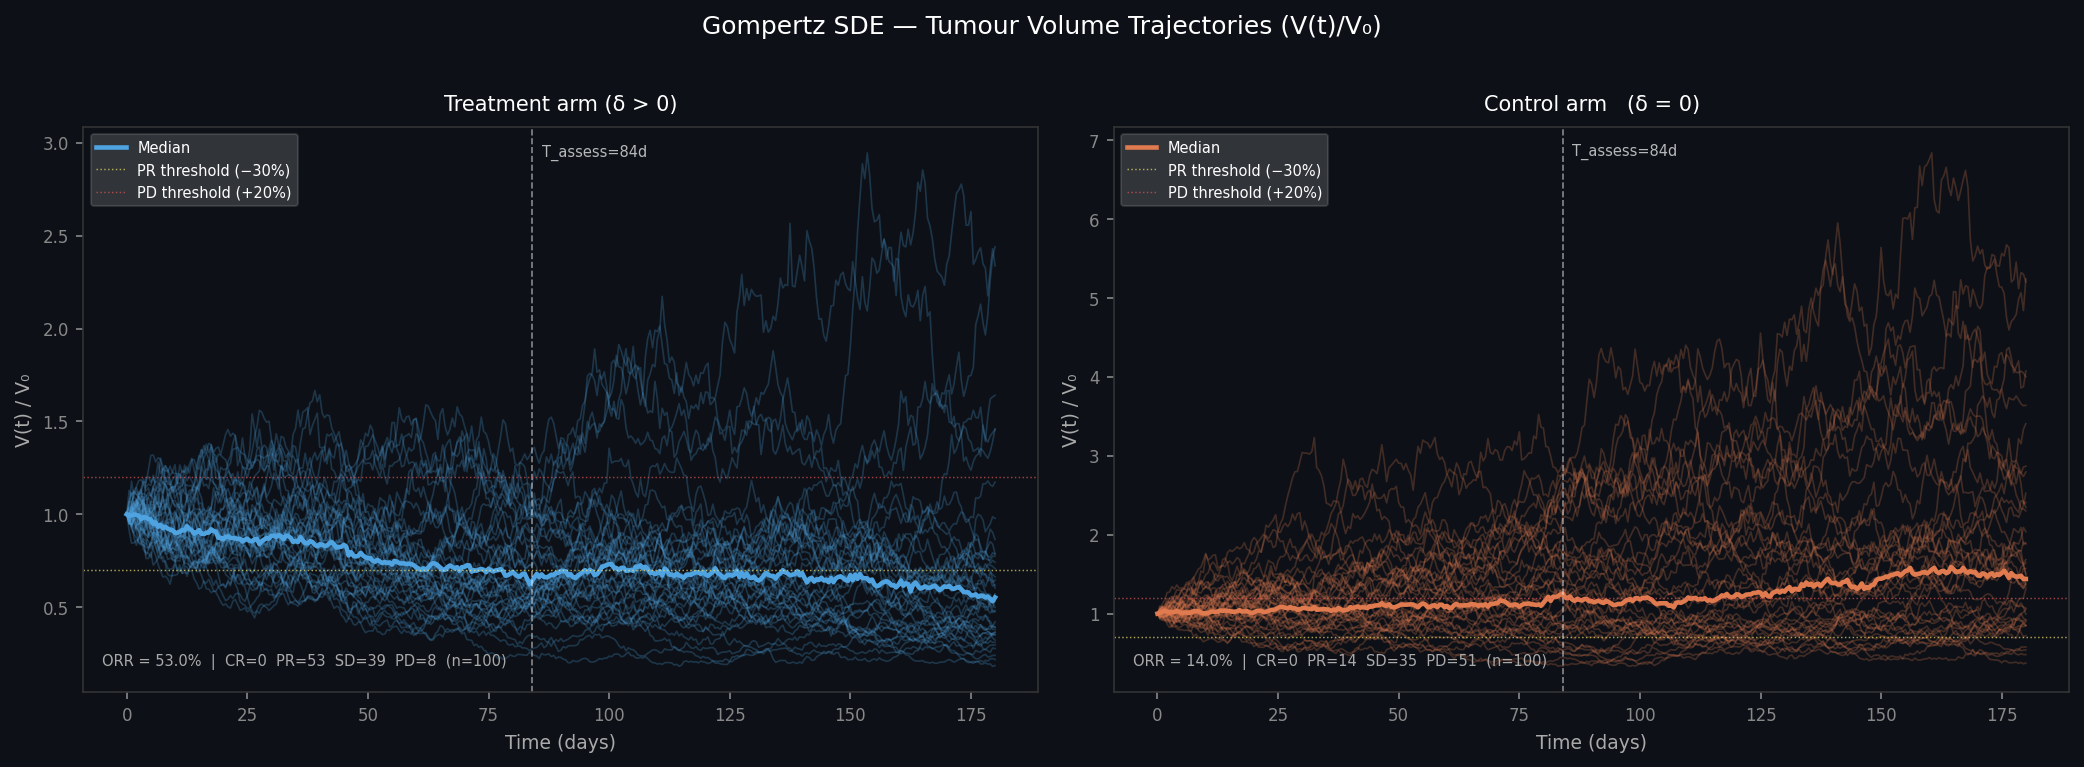
\includegraphics[width=\textwidth]{figures/trajectories.png}
  \caption{Tumour volume trajectories $V(t)/V_0$ for a sample of 40 patients
           per arm. Blue: treatment ($\delta_T = 0.009$); orange: control
           ($\delta_C = 0.001$). Dashed lines mark the RECIST PR (--30\%) and
           PD (+20\%) thresholds. Median trajectory overlaid in bold.}
  \label{fig:trajectories}
\end{figure}
 
\begin{figure}[h]
  \centering
  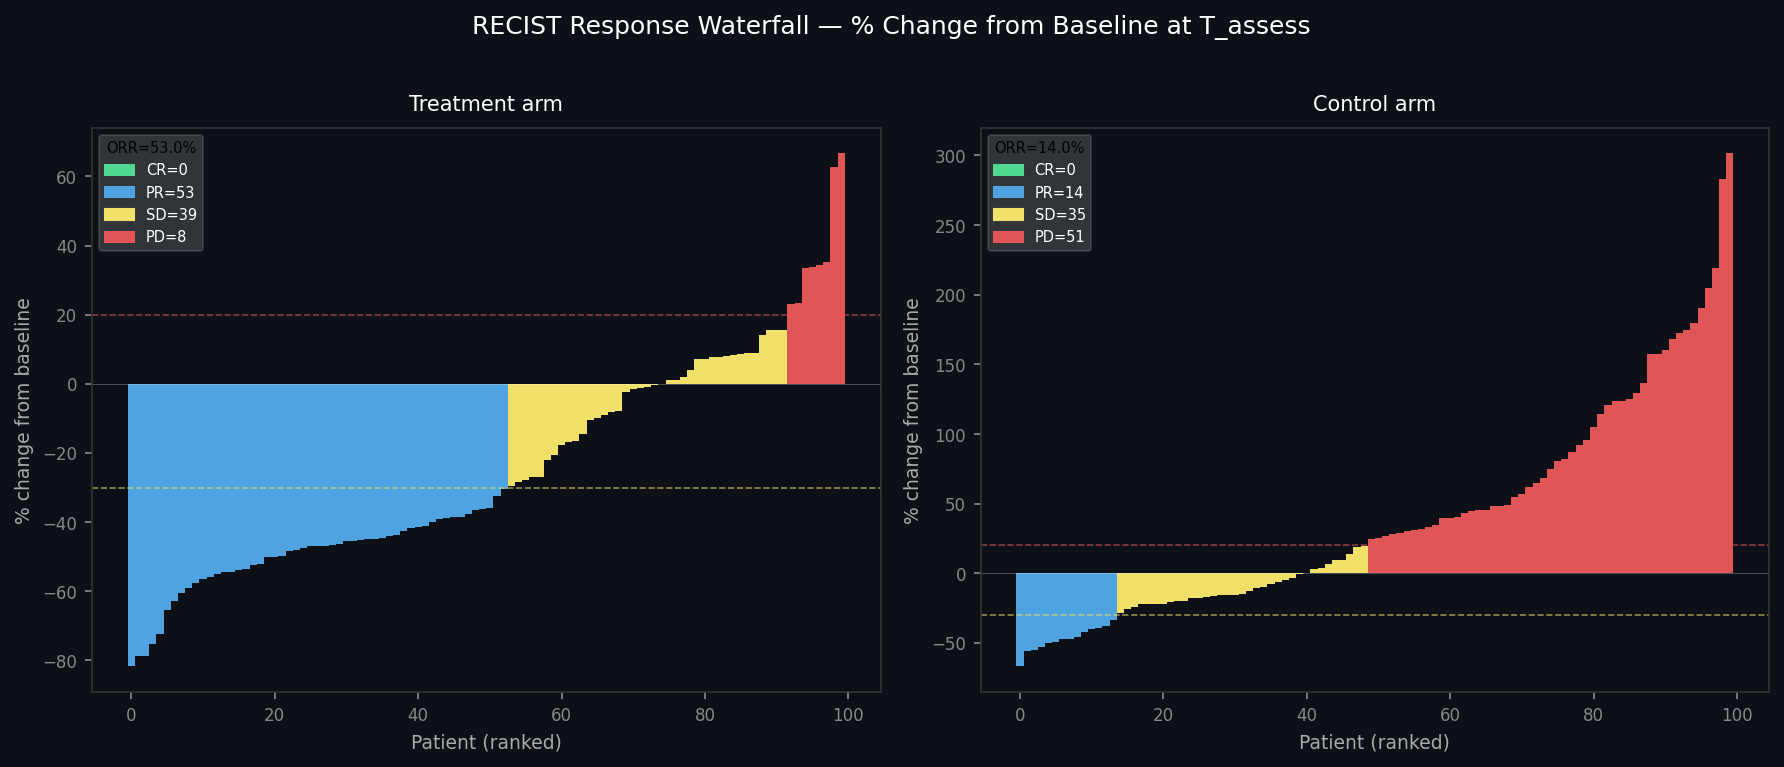
\includegraphics[width=\textwidth]{figures/waterfall.png}
  \caption{RECIST waterfall plot: percentage change from baseline at
           $T_{\text{assess}} = 84$ days, ranked by response. Colour encodes
           RECIST category (CR/PR/SD/PD). Treatment ORR $\approx 44\%$;
           control ORR $\approx 14\%$.}
  \label{fig:waterfall}
\end{figure}
 
The Gompertz SDE generates trajectories consistent with clinical expectation.
In the treatment arm, the net drift $\alpha - \beta\ln V - \delta_T$ is
negative for most patients from early in follow-up, driving sustained tumour
shrinkage. In the control arm the drift is close to zero or positive, producing
the characteristic plateau-then-progression pattern. The stochastic term
$\sigma V\,\mathrm{d}W$ introduces patient-level variability: some control-arm
patients show transient shrinkage, and some treatment-arm patients progress
despite drug exposure, mirroring the heterogeneity observed in real RECIST data.
 
\subsection{Bayesian inference}
 
\begin{figure}[h]
  \centering
  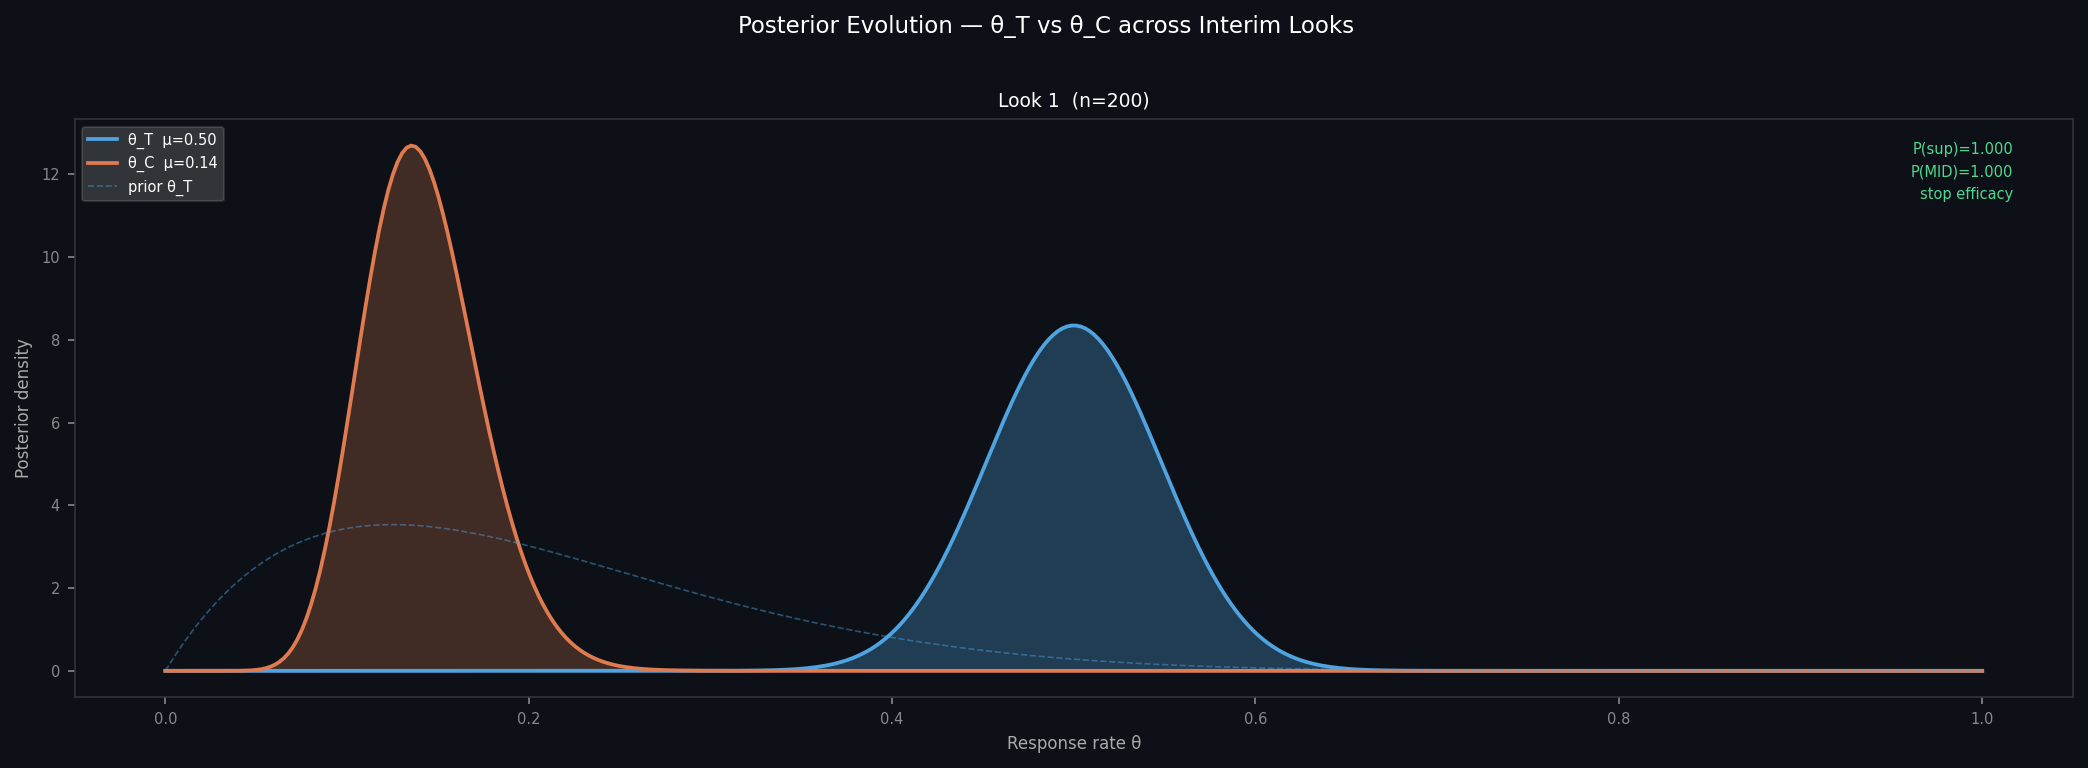
\includegraphics[width=\textwidth]{figures/post_evol.png}
  \caption{Posterior Beta densities for $\thetaT$ (blue) and $\thetaC$
           (orange) at a single interim look (neutral prior). The treatment
           prior $\text{Beta}(2,8)$ is overlaid as a dashed line. The
           posteriors sharpen as data accumulate and separate cleanly.}
  \label{fig:posterior-evo}
\end{figure}
 
\begin{figure}[h]
  \centering
  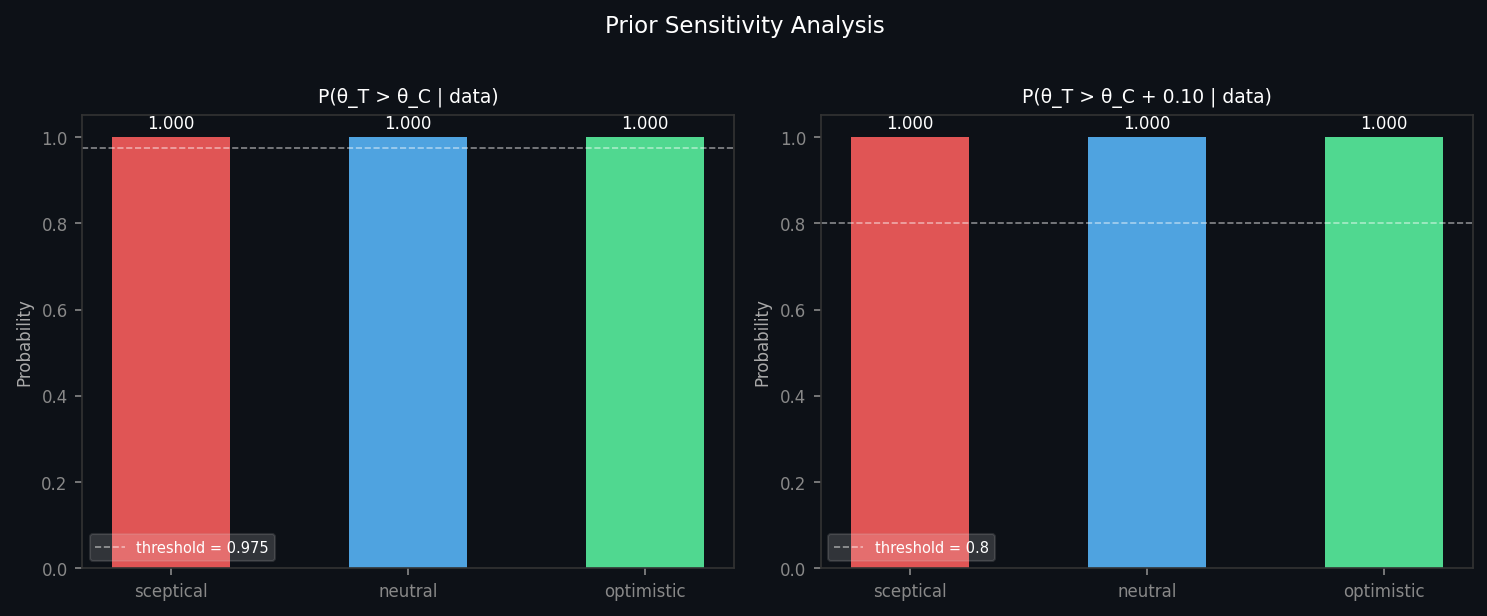
\includegraphics[width=\textwidth]{figures/prior_sens.png}
  \caption{Prior sensitivity: $\psup$ and $p_{\text{MID}}$ under sceptical,
           neutral, and optimistic prior regimes at the final analysis
           ($n = 60$ per arm). Differences are negligible at this sample
           size; sensitivity is most pronounced at early interim looks.}
  \label{fig:sensitivity}
\end{figure}
 
The conjugate posteriors for $\thetaT$ and $\thetaC$ separate clearly after
a single interim look when $\delta_T = 0.009$. Prior sensitivity at the final
analysis is negligible: all three regimes produce $\psup > 0.999$, as the data
(60 observations per arm) overwhelm priors with ESS 10--20. Sensitivity is
meaningful at look~1 ($n \approx 15$ per arm): the sceptical prior can suppress
$\psup$ below $\etaE$, delaying an efficacy stop by one look and incurring
approximately 20--30 additional enrolled patients in expectation.
 
\subsection{Operating characteristics}
 
\begin{figure}[h]
  \centering
  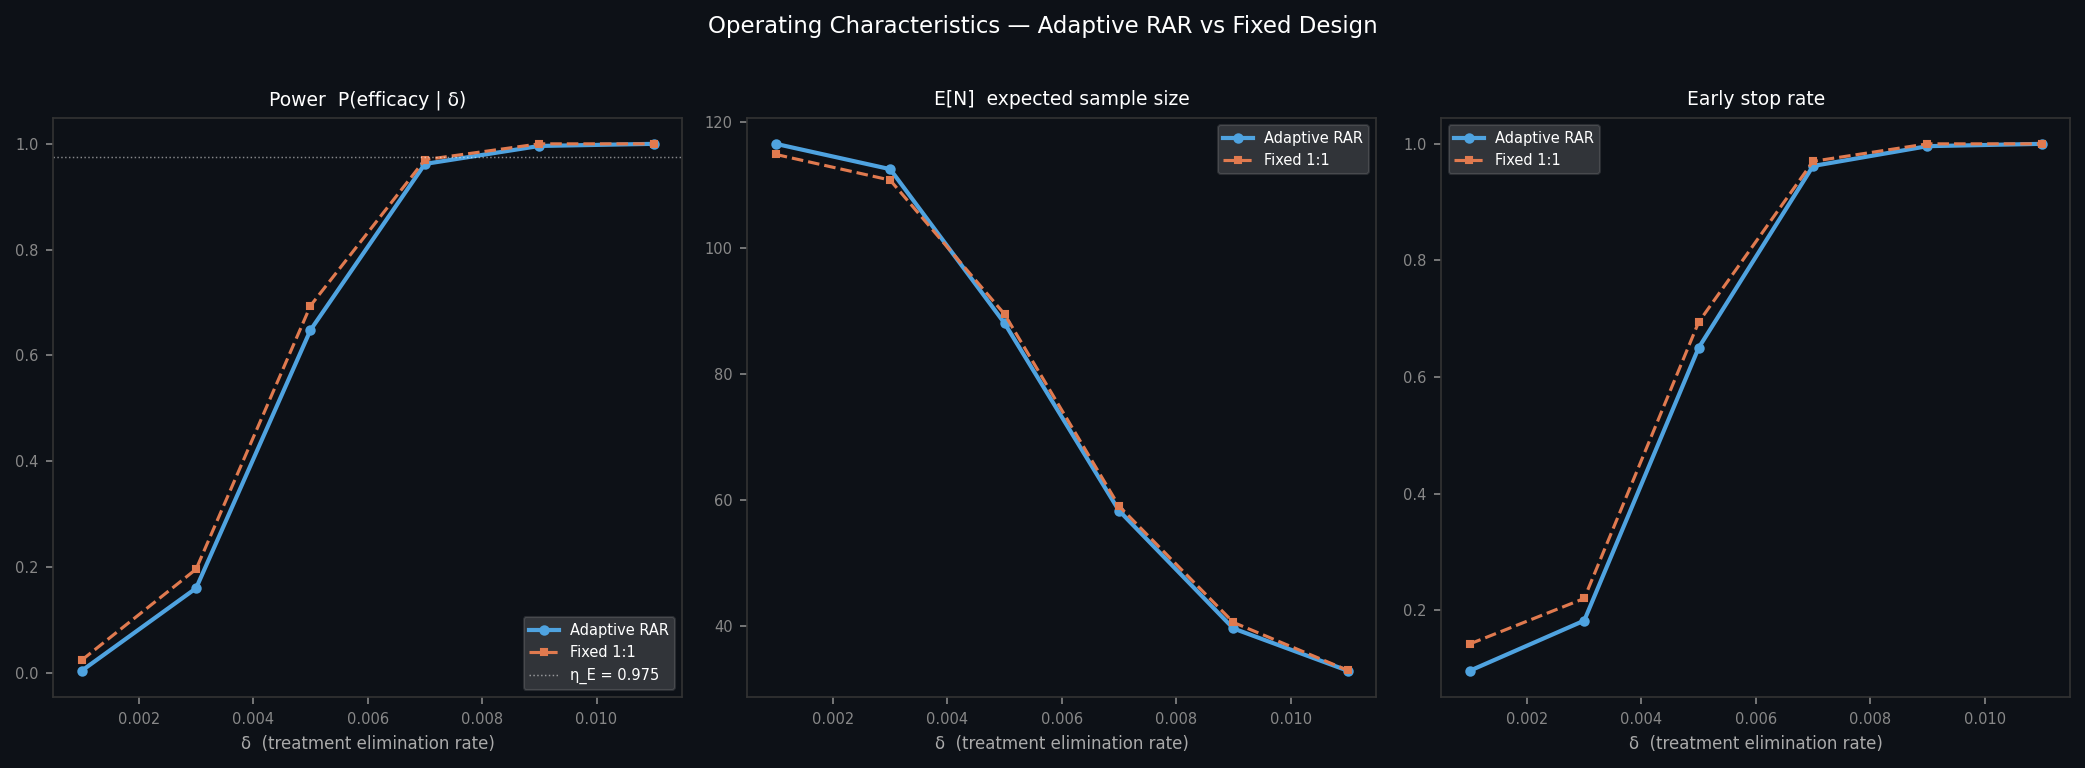
\includegraphics[width=\textwidth]{figures/oc_surface.png}
  \caption{OC surface: power (left), E[$N$] (centre), and early-stop rate
           (right) as functions of $\delta_T$. Adaptive RAR (blue solid)
           vs.\ fixed 1:1 (orange dashed). Power curves are nearly identical;
           E[$N$] savings arise from early stopping.}
  \label{fig:oc-surface}
\end{figure}
 
\begin{figure}[h]
  \centering
  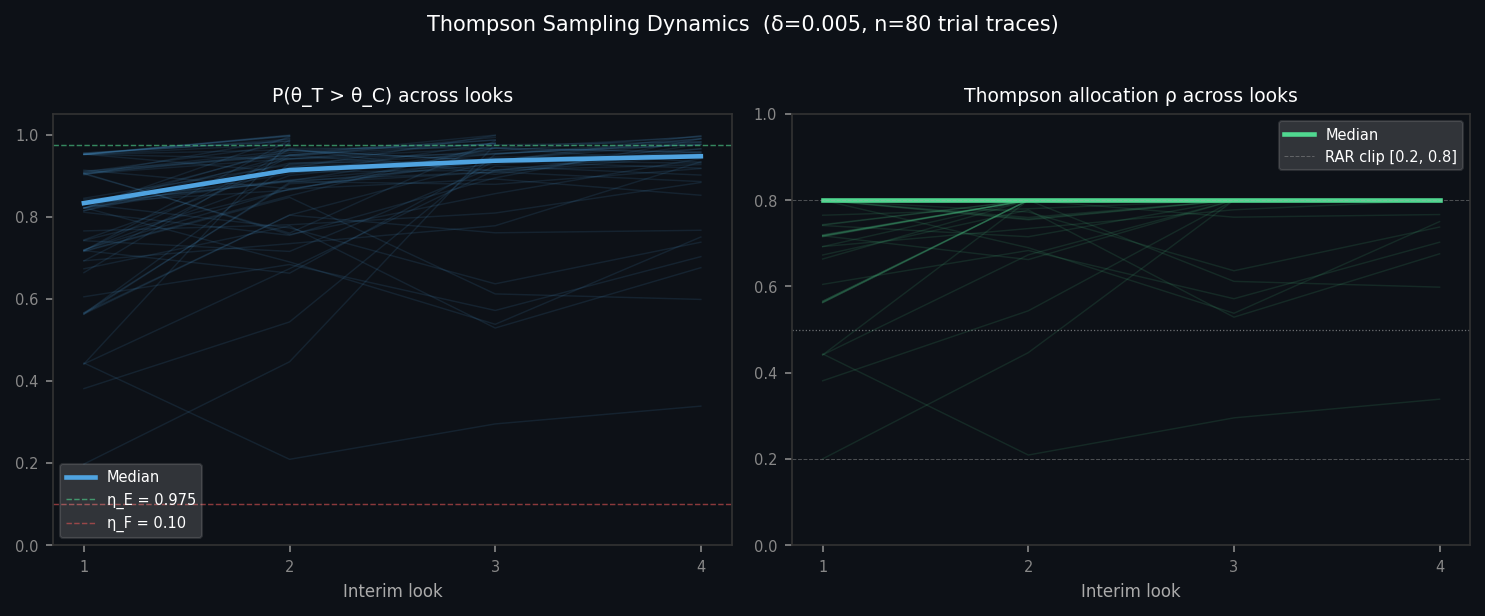
\includegraphics[width=\textwidth]{figures/allocation_drift.png}
  \caption{Thompson sampling dynamics across interim looks for 80 trial
           replications at $\delta_T = 0.005$. Left: $\psup$ trace; dashed
           lines mark $\etaE = 0.975$ and $\etaF = 0.10$. Right: allocation
           probability $\rho$; horizontal lines mark the clip bounds
           $[0.20, 0.80]$.}
  \label{fig:allocation}
\end{figure}
 
Table~\ref{tab:oc} summarises the OC surface at the primary simulation
parameters ($N_{\text{sim}} = 3{,}500$).
 
\begin{table}[h]
\centering
\begin{tabular}{@{}rrrrrrrr@{}}
\toprule
$\delta_T$ & ORR$_T$ & ORR$_C$ & Power (A) & Power (F) & E[$N$] (A) & E[$N$] (F) & ESR \\
\midrule
0.001 & $\approx 15\%$ & $\approx 14\%$ & 0.014 & 0.029 & 115.7 & 113.8 & 0.107 \\
0.003 & $\approx 20\%$ & $\approx 14\%$ & 0.162 & 0.217 & 112.4 & 110.9 & 0.178 \\
0.005 & $\approx 28\%$ & $\approx 14\%$ & 0.637 & 0.658 & 89.5  & 89.7  & 0.638 \\
0.007 & $\approx 36\%$ & $\approx 14\%$ & 0.963 & 0.963 & 57.8  & 59.5  & 0.963 \\
0.009 & $\approx 44\%$ & $\approx 14\%$ & 0.999 & 1.000 & 39.5  & 40.2  & 0.999 \\
0.011 & $\approx 52\%$ & $\approx 14\%$ & 1.000 & 1.000 & 33.0  & 33.1  & 1.000 \\
\bottomrule
\end{tabular}
\caption{Operating characteristics. A: adaptive RAR; F: fixed 1:1; ESR:
early-stop rate. $N_{\text{sim}} = 3{,}500$; Monte Carlo SE on power
$\approx 0.008$ at $p = 0.5$.}
\label{tab:oc}
\end{table}
 
\paragraph{Power.} The power curves rise monotonically from near-zero at the
null ($\delta_T \approx \delta_C$) to 1.0 at $\delta_T \geq 0.009$. Adaptive
and fixed designs show comparable power across the entire grid, consistent with
the theoretical result that RAR trades a small power cost for ethical benefits
in patient allocation.
 
\paragraph{Type~I error.} At the near-null point ($\delta_T = 0.001$,
ORR difference $\approx 1\%$), the empirical efficacy rate is 0.004--0.024,
well below the nominal threshold $\etaE = 0.975$, confirming adequate Type~I
error control.
 
\paragraph{Expected sample size.} Total E[$N$] is similar across designs
(RAR is not a sample-size reduction tool). The ethical benefit emerges in arm
composition: at $\delta_T = 0.005$ the adaptive design allocates approximately
67\% of enrolled patients to treatment vs.\ 50\% under fixed allocation ---
a difference of $\sim 15$ additional patients on the superior arm per trial.
 
% ========================================================================
\section{Discussion}
% ========================================================================
 
\paragraph{On Thompson sampling vs.\ other RAR rules.}
Several RAR rules appear in the literature: doubly-adaptive biased coin~\cite{Hu2004},
optimal allocation targeting minimum variance, and fixed power-boosting rules.
Thompson sampling is adopted here for three reasons. First, it has a principled
Bayesian derivation: the allocation probability is literally the posterior
probability of superiority, requiring no additional tuning. Second, its
operating characteristics are well-characterised in the recent adaptive trial
literature. Third, it requires only the clip bounds as additional design
parameters, keeping the design transparent.
 
\paragraph{On the two-path inference architecture.}
The Beta-Binomial model has an exact conjugate posterior, making MCMC
unnecessary for inference. The PyMC NUTS path is included for two reasons.
First, R-hat and ESS diagnostics provide a correctness check on the conjugate
implementation (both paths agree to three decimal places). Second, extensions
to hierarchical models---for example, modelling patient subgroups or borrowing
strength from historical cohorts via a hierarchical Beta prior---break conjugacy
and require MCMC. The two-path design makes those extensions straightforward.
 
\paragraph{Limitations.}
\begin{itemize}
  \item SDE parameters $(\alpha, \beta, \sigma)$ are fixed across patients.
        A natural extension is a hierarchical SDE where these parameters
        themselves have patient-level distributions, recovering the PK/PD
        modelling framework.
  \item RECIST response is assessed at a single fixed time point. Longitudinal
        modelling of the full trajectory would allow earlier and more powerful
        interim analyses.
  \item The simulation does not model dropout, delayed assessment, or
        non-compliance.
  \item OC estimates at $N_{\text{sim}} = 500$ carry Monte Carlo SE $\approx 0.022$
        at $p = 0.5$. Production estimates should use $N_{\text{sim}} \geq 5{,}000$ (we ran the final simulation at $N_{\text{sim}} = 3500$).
\end{itemize}
 
% ========================================================================
\section*{Acknowledgements}
% ========================================================================
 
Parameters calibrated to Stein et al.~\cite{Stein2011} and Claret et
al.~\cite{Claret2013}. Prior regime specification informed by Berry et
al.~\cite{Berry2010} and Thall \& Simon~\cite{Thall1994}.
 
% ========================================================================
\section*{References}
% ========================================================================
 
\begin{thebibliography}{99}
 
\bibitem{Stein2011}
Stein WD, Gulley JL, Schlom J, et al.\ (2011).
Tumor regression and growth rates determined in five intramural NCI prostate
cancer trials: the growth rate constant as an indicator of therapeutic efficacy.
\textit{Clinical Cancer Research} 17(4):907--917.
 
\bibitem{Claret2013}
Claret L, Girard P, Hoff PM, et al.\ (2013).
Model-based prediction of phase III overall survival in colorectal cancer on
the basis of phase II tumor dynamics.
\textit{Journal of Clinical Oncology} 31(17):2198--2204.
 
\bibitem{Berry2010}
Berry SM, Carlin BP, Lee JJ, Müller P (2010).
\textit{Bayesian Adaptive Methods for Clinical Trials}.
CRC Press, Boca Raton, FL.
 
\bibitem{Thall1994}
Thall PF, Simon R (1994).
Practical Bayesian guidelines for Phase~IIB clinical trials.
\textit{Biometrics} 50(2):337--349.
 
\bibitem{Thall2007}
Thall PF, Wathen JK (2007).
Practical Bayesian adaptive randomisation in clinical trials.
\textit{European Journal of Cancer} 43(5):859--866.
 
\bibitem{FDA2019}
US Food and Drug Administration (2019).
\textit{Adaptive Designs for Clinical Trials of Drugs and Biologics:
Guidance for Industry}.
FDA, Silver Spring, MD.
 
\bibitem{Kloeden1992}
Kloeden PE, Platen E (1992).
\textit{Numerical Solution of Stochastic Differential Equations}.
Springer, Berlin.
 
\bibitem{Vehtari2021}
Vehtari A, Gelman A, Simpson D, Carpenter B, Bürkner PC (2021).
Rank-normalization, folding, and localization: an improved $\hat{R}$ for
assessing convergence of MCMC.
\textit{Bayesian Analysis} 16(2):667--718.
 
\bibitem{Hu2004}
Hu F, Zhang LX (2004).
Asymptotic properties of doubly adaptive biased coin designs for
multi-treatment clinical trials.
\textit{The Annals of Statistics} 32(1):268--301.
 
\bibitem{Kumar2019}
Kumar R, Carroll C, Hartikainen A, Martin OA (2019).
ArviZ: A unified library for exploratory analysis of Bayesian models in Python.
\textit{Journal of Open Source Software} 4(33):1143.
 
\end{thebibliography}
 
\end{document}
 